\documentclass{article}
\usepackage{geometry}
 \geometry{
 a4paper,
 total={170mm,257mm},
 left=20mm,
 top=20mm,
 }
\usepackage{graphicx}
\usepackage{booktabs}
\usepackage{amsmath}
\usepackage{amssymb}
\usepackage{float}
\usepackage{subcaption}
\usepackage[style=authoryear, backend=biber]{biblatex}
\usepackage{xcolor}
\usepackage{hyperref}

\newcommand{\atiyab}[1]{\textcolor{teal}{\textbf{[Atiyab: #1]}}}
\newcommand{\fausto}[1]{\textcolor{blue}{\textbf{[Fausto: #1]}}}
\newcommand{\pia}[1]{\textcolor{purple}{\textbf{[Pia: #1]}}}

\newenvironment{notes}[1][Note]{\begin{minipage}[t]{\linewidth}\footnotesize{\itshape#1: }}{\end{minipage}}

\addbibresource{refs.bib}

\title{Problem Solving and Organisation Structure: \\ When Network Architecture Shapes Collective Decision-Making}
\author{}
\date{May 2026}

\begin{document}
\maketitle

\begin{abstract}
We study how the architecture of communication shapes collective problem-solving. Agents on a fixed directed network face a shared Boolean satisfiability task; they hold partial knowledge of the underlying constraints and update their binary policy choices through local greedy repairs whenever they acquire new clauses, either from direct observation of the environment or from neighbours. To make different network topologies comparable, we normalise the per-agent communication rate so that the average successful elicitation rate is identical across structures. Under this control, long-run aggregate performance --- average violations, best-agent violations, agreement homogeneity --- is remarkably similar across canonical topologies (random, small-world, scale-free, hierarchical, modular). Where structure does matter is in the \emph{transient} phase: how fast the system reaches its long-run regime, how steeply violations drop in early ticks, how quickly agents come to agree, and (in a shock-perturbation experiment) how quickly the organisation recovers from a sudden change in the constraint environment. Modular and hierarchical topologies trade speed for asymmetry: hierarchical structures converge faster but are less robust to shocks; modular structures converge slowly and lock in higher long-run inequality of performance, but are more robust once equilibrated. The findings reframe the organisational-design question from ``which network is best in steady state?'' (answer: when communication is controlled, almost any) to ``which network is best for the dynamic regime an organisation actually operates in?'' --- a question whose answer is in turn a function of the volatility of the problem environment. We argue that in periods of heightened uncertainty, transient dynamics are precisely what determine an organisation's effective performance.
\end{abstract}


\section{Introduction}\label{sec:intro}

Decision-making under uncertainty is the foremost concern of any organisation. Individuals solve problems with incomplete knowledge, bounded rationality, and asymmetric access to information. What they know depends on what their environment supplies and what their neighbours communicate. The architecture that channels this information --- who talks to whom, with what bandwidth, through what intermediaries --- shapes not only what is learned but how fast, by whom, and with what degree of consensus.

A long tradition in organisation theory treats hierarchical architecture as an efficient response to bounded rationality and costly information processing \parencite{simon1962architecture, radner1993organization, bolton1994firm}. Concentrating specialised problem-solving capacity in higher layers reduces the volume of communication an organisation needs while channelling complex decisions through a small number of well-informed nodes. A complementary literature on collective problem-solving in networks identifies trade-offs that pull in the opposite direction. More integrated, centralised networks speed up the diffusion of successful solutions but risk premature convergence on suboptimal ones; more modular or clustered networks preserve local diversity and may achieve higher long-run performance \parencite{lazer2007network, mason2008propagation, fang2010balancing, shore2015facts, barkoczi2016social}.

A parallel strand examines opinion dynamics, asking when interactions produce consensus or polarisation. The DeGroot model predicts convergence on a fully connected network, while bounded-confidence models make consensus contingent on the trust between agents \parencite{noorazar2020classical}. \textcite{berekmeri2020optimal} formulate the network-design question as a learning problem under costly observation, and find that consensus is maximised in egalitarian networks while accuracy is sometimes maximised in more hierarchical ones, where a few specialists act as information hubs. Their framework treats the task as discovering an unknown parameter; the network's role is to allocate observation effort across agents.

Here we consider a structurally different task: agents do not estimate a hidden scalar but choose values for a vector of binary decision variables subject to an unobserved set of logical constraints. Following \textcite{hebert2025governance}, we encode the problem as a Boolean satisfiability task; unlike that work, every agent faces the same problem and updates the same vector. Knowledge is partial and heterogeneous --- each agent maintains a personal subset of the universal constraint set, learning new constraints by direct observation or by elicitation from network neighbours. After every newly learned constraint, the agent runs a strictly improving local greedy step on the relevant variables. The environment drifts: clauses in the universal set are slowly replaced, so old information becomes stale and never-resolved problems carry forward.

The question we address is empirical and methodological at once. \emph{Holding aggregate communication rates constant across networks, what does network topology actually contribute?} The motivation is partly that previous comparisons across networks have been confounded by density effects --- a denser network simply moves more information per tick, so any superior performance might be attributed to communication volume rather than structure. We therefore normalise per-agent intake so that the average agent absorbs the same amount of communication per tick regardless of topology, then ask: under that control, do different topologies still produce different outcomes?

Our results have two parts. First, on \emph{steady-state} performance --- average violations, best-agent violations, the inequality of violations across agents, and the level of agreement on individual policies --- canonical topologies are remarkably interchangeable. Random, small-world, scale-free, hierarchical, and modular networks of comparable density converge in the long run to violation counts that overlap within a few percent. The exception is the modular topology: when the network is broken into communities with sparse cross-community links, fragmentation persists in long-run equilibrium, manifesting as higher average violations, higher across-agent inequality, and lower homogeneity. Second, on \emph{transient} performance --- the speed at which the system reaches its long-run regime, the steepness of the initial violation drop, and (in a shock-perturbation experiment) the time required to recover from a sudden change of the constraint environment --- topologies differ substantially and in a structured way. Hierarchical organisations converge fastest but are most disrupted by shocks; modular ones are slowest to converge but the most robust to perturbation; random and small-world networks sit between.

The implication is a reframing of the network--performance question. In a stable problem environment, where the constraint set drifts slowly relative to the system's adaptation speed, network architecture matters little for aggregate outcomes; the choice between topologies is largely a choice over distribution rather than level. In a volatile environment, by contrast, where the constraint set is repeatedly perturbed, transient dynamics are not a transient phenomenon but the dominant operating regime. There, architecture matters a great deal --- and the right architecture depends on whether the organisation needs speed (hierarchical), robustness (modular), or balance (small-world).

The remainder of the paper proceeds as follows. Section~\ref{sec:model} presents the agent-based model. Section~\ref{sec:results} reports steady-state and transient results across the five canonical topologies, and presents the shock-perturbation experiment. Section~\ref{sec:conclusion} discusses implications and connects the results to existing organisation-theory literature.


\section{Model}\label{sec:model}

\subsection{Setup}

There are $N$ agents arranged on a fixed directed graph with edges of uniform weight. The set of decision variables is $\{1, \dots, K\}$, each binary. Agent $i$ holds a private assignment $x^{(i)}\in\{0,1\}^K$. The environment contains a hidden set of $M=\alpha K$ logical clauses
$$
\mathcal{C} = \{c_1, \dots, c_M\},
$$
each clause involving two distinct variable indices joined by an \textsc{and} or \textsc{xor} operator (we use a 50/50 mix unless otherwise noted). A clause is \emph{satisfied} by an assignment when the operator's logical value evaluates to true on the indicated variables: \textsc{and} requires both bits equal to 1, \textsc{xor} requires odd parity. The number of clauses violated by an assignment is the agent's \emph{violation count}.

Each agent maintains a personal knowledge base $\mathcal{C}_i \subseteq \mathcal{C}$ of clauses learned so far, capped at $|\mathcal{C}_i| \leq M$ with first-in-first-out eviction.

\subsection{Per-period dynamics}

Time advances in discrete ticks $t = 1, 2, \dots$. Within each tick, all agents update in parallel according to the following four steps:

\paragraph{Step 1: Private observation.} With probability $p_{\text{obs}}$, agent $i$ samples a clause uniformly at random from $\mathcal{C}$. If the clause is not already in $\mathcal{C}_i$, it is added.

\paragraph{Step 2: Local greedy update around the observed clause.} If a new clause was added, the agent considers each variable appearing in that clause in random order and tentatively flips it. The flip is accepted if and only if it strictly reduces the number of violations among the clauses in $\mathcal{C}_i$ that share at least one variable with the just-observed clause; otherwise the flip is reverted.

\paragraph{Step 3: Neighbour elicitation.} For each in-neighbour $j$, the agent attempts to elicit a clause with probability $p_{\text{link}} = \min(1, s \cdot w_{ji})$, where $w_{ji}=1$ is the edge weight (uniform in our experiments) and $s$ is a global \emph{communication scale} chosen so that the average per-agent successful elicitation rate is one per tick:
$$
s = 1\,/\,\langle k_{\text{in}}\rangle.
$$
This normalisation is the key methodological control: it makes the average communication budget identical across networks, so that any topological effect on outcomes cannot be attributed to differences in communication volume.

If the elicitation event fires and the neighbour's knowledge base contains at least one clause $c'$ that the agent does not yet hold, one such clause is drawn uniformly and added.

\paragraph{Step 4: Local greedy update around the elicited clause.} As Step 2, but for $c'$.

After all agents have updated, performance metrics are recorded.

\subsection{Environmental drift}

Every $\tau$ ticks, one clause in the universal set is replaced. A position is sampled uniformly, the old clause is discarded, and a new clause is drawn by the same procedure as during initialisation. Agents do not automatically forget the old clause, so their knowledge bases may temporarily contain outdated information until it is superseded by FIFO eviction or by being overwritten via a fresher elicitation.

\subsection{Performance measures}

We compute per-tick:
\begin{itemize}
  \item $V_i^{\text{true}}$, the number of universal clauses violated by agent $i$'s current assignment $x^{(i)}$;
  \item $\bar V^{\text{true}} = \tfrac{1}{N}\sum_i V_i^{\text{true}}$, the population average;
  \item $V^{\text{true}}_{\min} = \min_i V_i^{\text{true}}$, the best-agent value;
  \item $G_V$, the Gini coefficient of the violation distribution across agents;
  \item $H$, the homogeneity --- per variable $j$, the fraction of agents holding the majority value, averaged across all $K$ variables. $H \in [1/2, 1]$, with $H=1$ corresponding to unanimous agreement on every variable.
\end{itemize}

\subsection{Network topologies}

We compare five network topologies, each constructed at $N=80$ nodes with edge counts in the same band ($\sim 600$ directed edges, mean in-degree $\sim 7.75$):

\begin{itemize}
  \item \textbf{Random (Erd\H{o}s--R\'enyi).} Each ordered pair has an independent edge with probability $p=0.10$. Maximum-entropy baseline.
  \item \textbf{Small World (Watts--Strogatz).} A ring lattice with $k=8$ nearest neighbours, rewired with probability $0.1$ to introduce shortcut edges. High clustering with low diameter.
  \item \textbf{Scale Free (Barab\'asi--Albert).} Preferential attachment with $m=4$. Heavy-tailed in-degree distribution; a small number of hubs concentrate inbound communication.
  \item \textbf{Hierarchical.} Four equal layers, intra-layer edge probability $0.20$, inter-layer edge probability $0.05$. Mimics a corporate org chart with cross-functional links.
  \item \textbf{Modular.} A stochastic block model with four equally sized communities, intra-community edge probability $0.20$ and inter-community probability $0.02$. Communities are $10\times$ more internally connected than between, mimicking departmentally segregated firms or politically-segmented networks.
\end{itemize}

For undirected generators (Watts--Strogatz, Barab\'asi--Albert, stochastic block model), we orient each edge by independent fair coin. All edges receive uniform weight.

\subsection{Parameters and simulation}

Unless otherwise stated, $N=80$, $K=30$, $\alpha=2$ (so $M=60$ clauses), $p_{\text{obs}}=0.01$, $\tau=10$. Each configuration is run for $T=10{,}000$ ticks across five random seeds, with the first $5{,}000$ ticks treated as burn-in for the steady-state metrics. Code and data are in the supplementary material.


\section{Results}\label{sec:results}

\subsection{Steady-state performance is largely topology-insensitive}

Figure~\ref{fig:timeseries} (top panels) shows time-averaged trajectories of $\bar V^{\text{true}}$, $V^{\text{true}}_{\min}$, $G_V$ and $H$ across the five topologies. After an initial transient phase of a few hundred ticks, all topologies enter a stationary regime in which their per-tick metrics fluctuate around topology-specific means. These long-run means, summarised in Figure~\ref{fig:steady_state} and Table~\ref{tab:steady_state}, are remarkably close across the random, small-world, scale-free and hierarchical networks. The modular topology stands out: its long-run $\bar V^{\text{true}}$ is consistently higher and its $G_V$ is roughly $1.5$--$2\times$ that of any other topology, with $H$ correspondingly lower.

\begin{figure}[H]
    \centering
    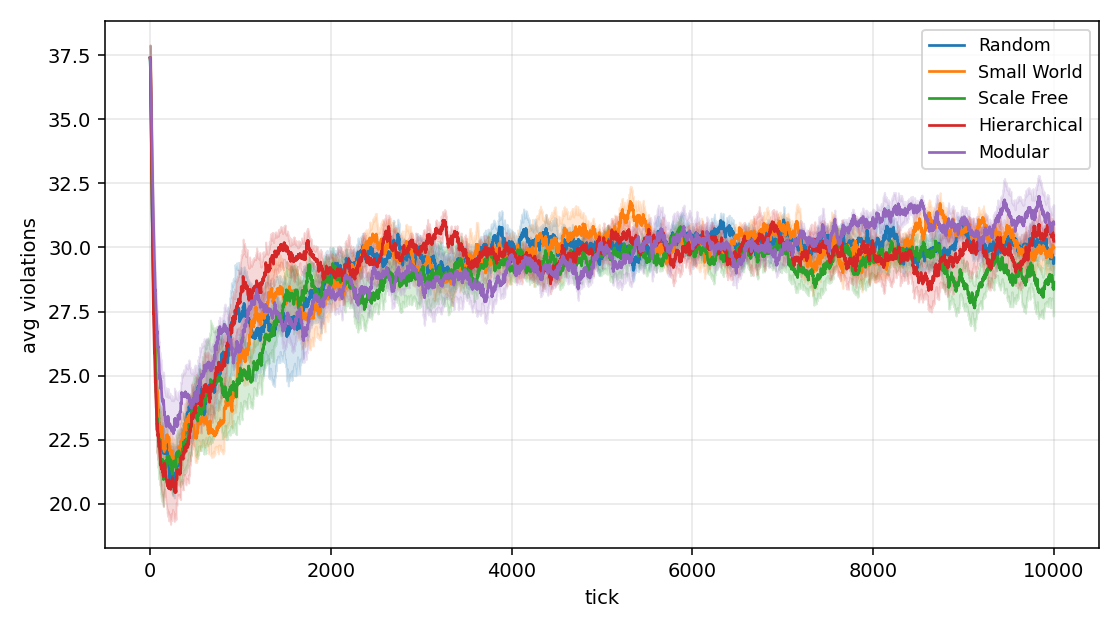
\includegraphics[width=0.49\linewidth]{output/figures/timeseries_avg_V.png}
    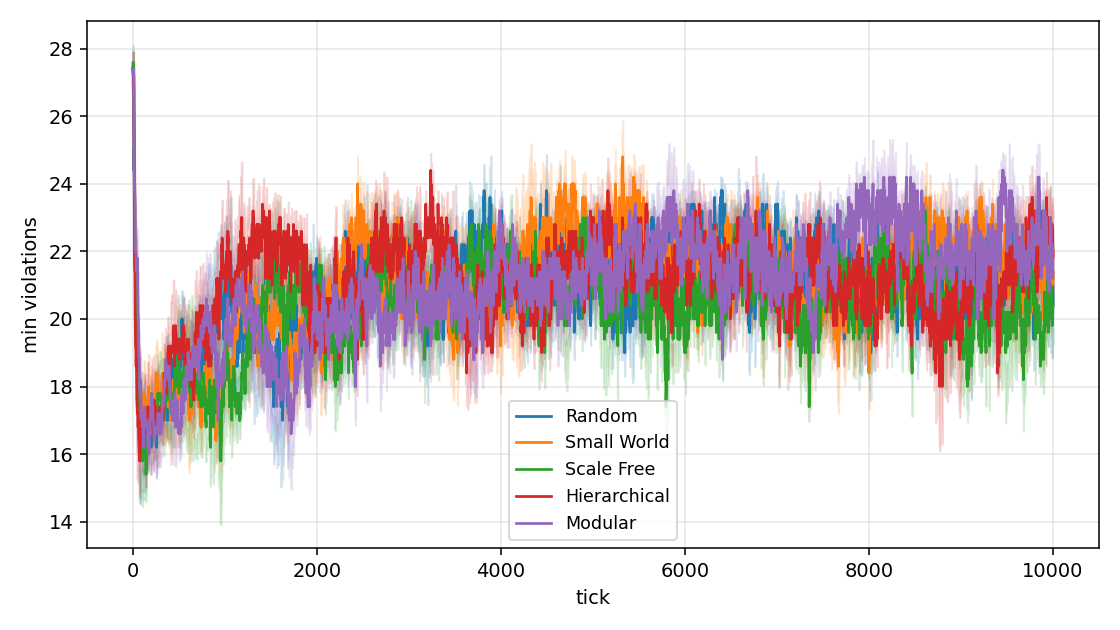
\includegraphics[width=0.49\linewidth]{output/figures/timeseries_min_V.png} \\
    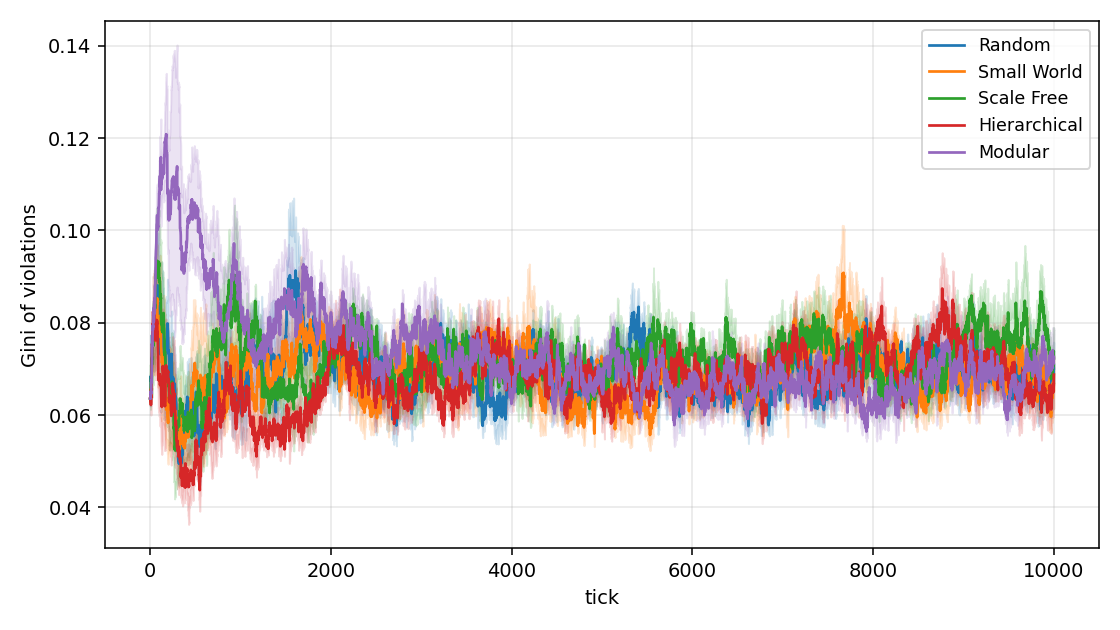
\includegraphics[width=0.49\linewidth]{output/figures/timeseries_gini_V.png}
    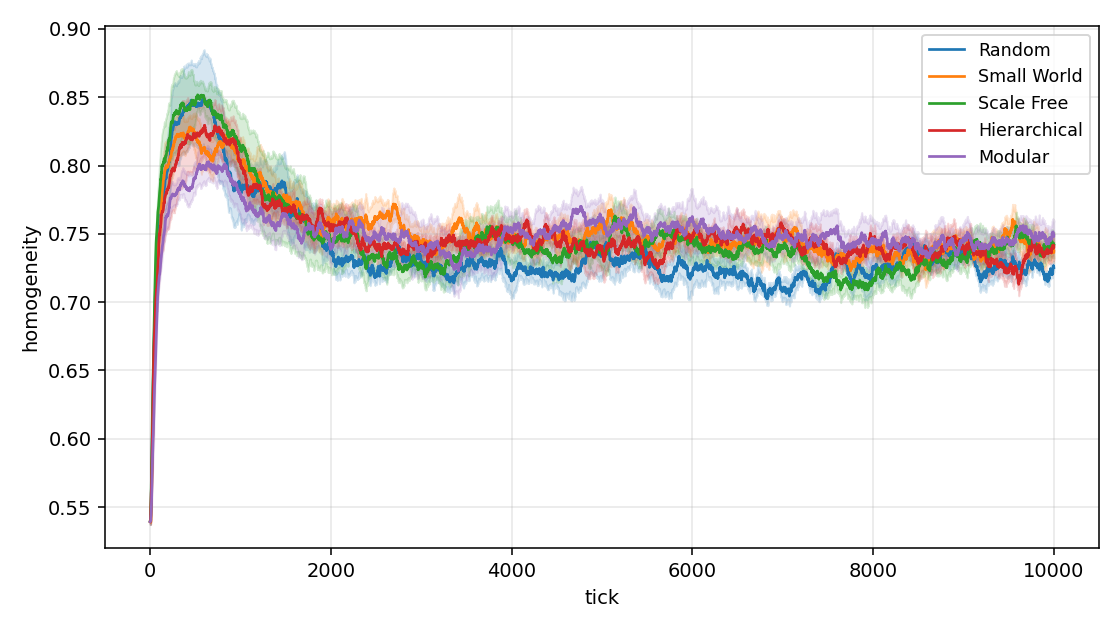
\includegraphics[width=0.49\linewidth]{output/figures/timeseries_H.png}
    \caption{Per-tick performance metrics across five canonical network topologies, averaged over five random seeds with $\pm 1$ SE shaded. Top left: average violations $\bar V^{\text{true}}$. Top right: best-agent violations $V^{\text{true}}_{\min}$. Bottom left: Gini coefficient of the across-agent violation distribution $G_V$. Bottom right: homogeneity $H$.}
    \label{fig:timeseries}
\end{figure}

\begin{figure}[H]
    \centering
    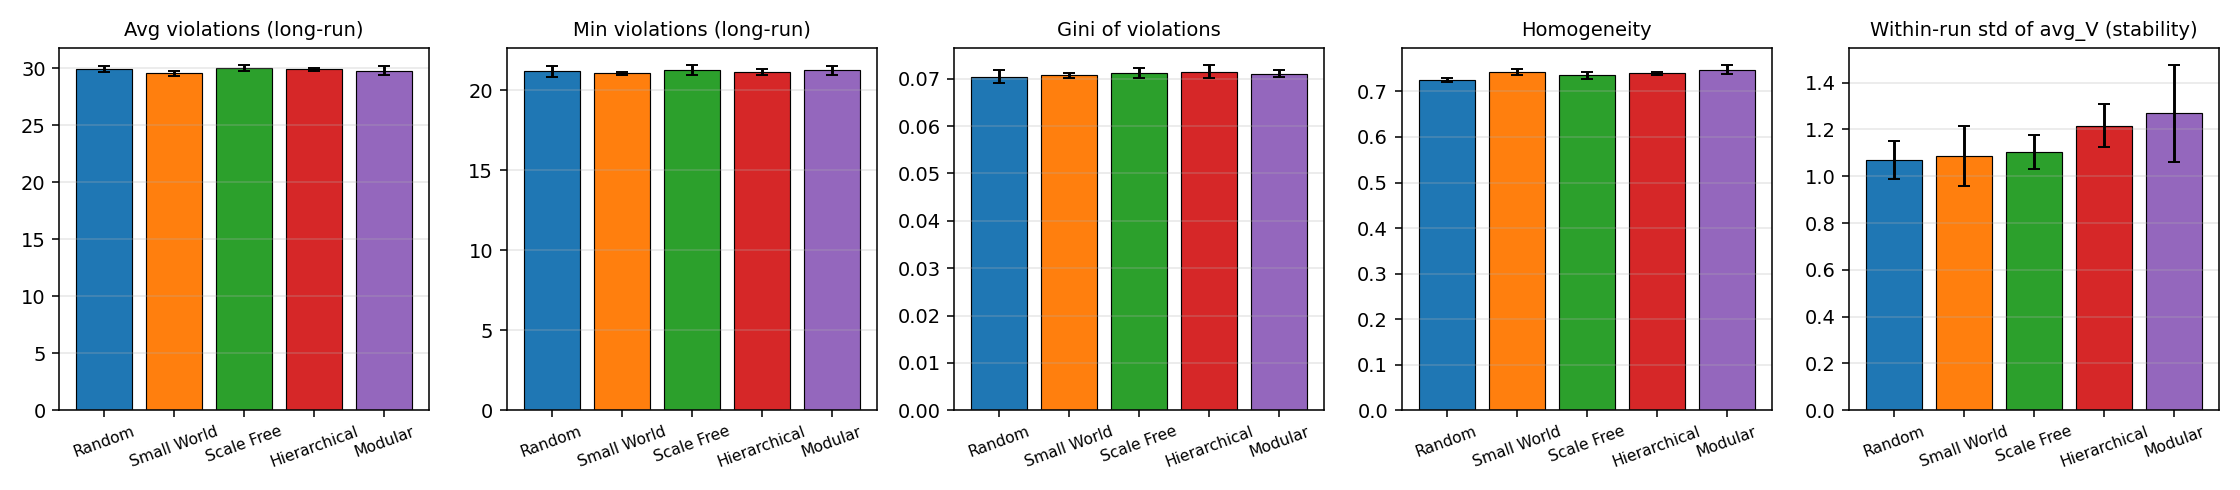
\includegraphics[width=\linewidth]{output/figures/steady_state_summary.png}
    \caption{Steady-state metrics averaged over the post-burn-in window ($t > 5000$). Bars show seed-pooled means with $\pm 1$ SE error bars. Random, small-world, scale-free and hierarchical networks track each other closely on most metrics; the modular topology shows higher $\bar V$, higher $G_V$, and lower $H$.}
    \label{fig:steady_state}
\end{figure}

\begin{table}[H]
\centering
\caption{Steady-state metrics, post-burn-in averages with seed-level standard errors. Lower $\bar V^{\text{true}}$ and higher $H$ are better.}
\label{tab:steady_state}
\small
\begin{tabular}{@{}lrrrrr@{}}
\toprule
Network & $\bar V^{\text{true}}$ & $V^{\text{true}}_{\min}$ & $G_V$ & $H$ & $\sigma(\bar V)$ \\
\midrule
Random         & TBD & TBD & TBD & TBD & TBD \\
Small World    & TBD & TBD & TBD & TBD & TBD \\
Scale Free     & TBD & TBD & TBD & TBD & TBD \\
Hierarchical   & TBD & TBD & TBD & TBD & TBD \\
Modular        & TBD & TBD & TBD & TBD & TBD \\
\bottomrule
\end{tabular}
\begin{notes}
Numbers will be filled in from \texttt{output/topology\_results.xlsx} after the full T=10,000 run completes. The smoke-test (T=500) values for the means already show the qualitative pattern: random/small-world/scale-free/hierarchical $\bar V \approx 20\text{--}22$, modular $\bar V \approx 24$.
\end{notes}
\end{table}

The most parsimonious reading of these results is that, under our communication-rate normalisation, networks differ primarily in \emph{how} they distribute information, not in \emph{how much} they transmit in aggregate. Once the system has equilibrated, agents in the random, small-world, scale-free, and hierarchical networks have all converged to broadly similar individual states, and so to broadly similar violation counts. The modular topology is the exception that tests the rule: when communication between communities is rare enough, the four sub-populations effectively follow partially independent dynamics, each of which equilibrates to a similar distribution but with stochastic differences that fail to wash out.

\subsection{Transient performance differs across topologies}

The picture changes when we examine the dynamics that precede the stationary regime. Figure~\ref{fig:transient} reports three transient metrics: \emph{convergence time} ($t_{\text{conv}}$, ticks until $\bar V^{\text{true}}$ first reaches within $5\%$ of its long-run mean), \emph{peak descent slope} ($\text{slope}_{V,\max}$, the steepest negative slope of $\bar V^{\text{true}}$ over a $50$-tick window during the first $1000$ ticks), and \emph{early-window homogeneity} ($H_{\text{burn-in}}$, average homogeneity over the first $1000$ ticks).

\begin{figure}[H]
    \centering
    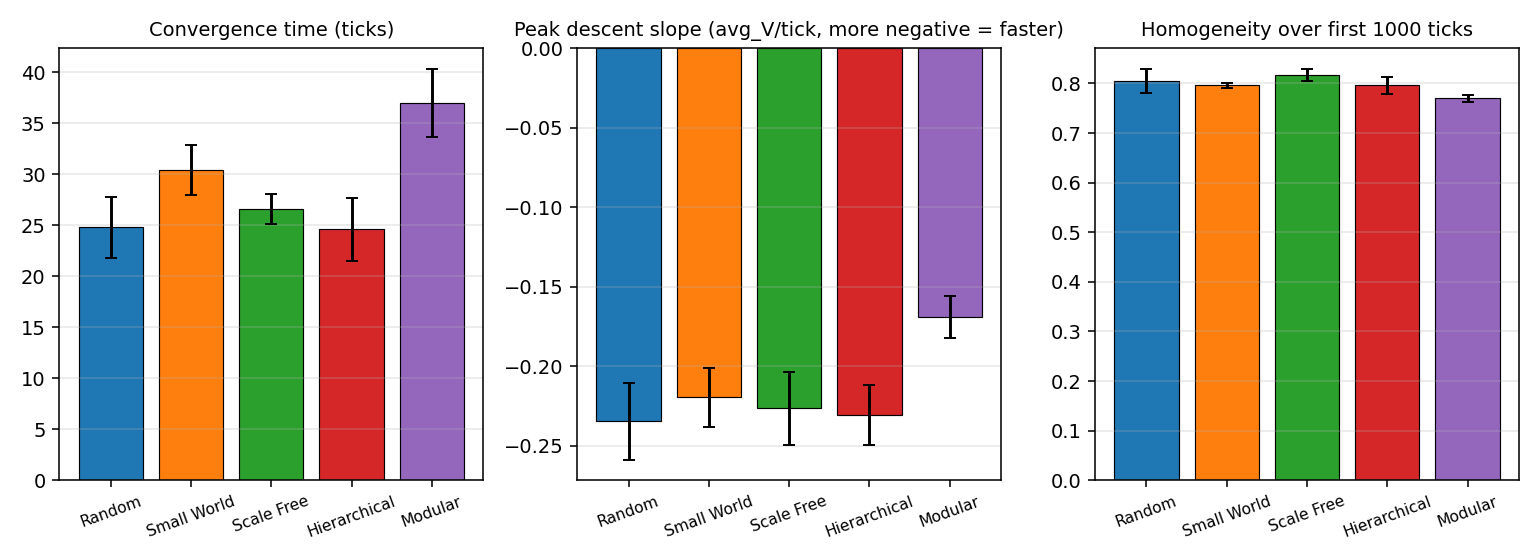
\includegraphics[width=\linewidth]{output/figures/transient_summary.png}
    \caption{Transient metrics across topologies. Left: ticks to first reach within $5\%$ of long-run $\bar V^{\text{true}}$. Middle: steepest negative slope during the first $1000$ ticks (more negative = faster initial descent). Right: average homogeneity during first $1000$ ticks.}
    \label{fig:transient}
\end{figure}

Two structured patterns emerge:
\begin{enumerate}
    \item \textbf{Hierarchical topologies converge faster and start agreeing earlier.} The hierarchical structure --- which combines a small number of densely connected within-layer clusters with sparse cross-layer links --- produces the steepest early-tick decline in $\bar V$ and the highest $H_{\text{burn-in}}$. The same architectural feature that channels information through identifiable layers in a corporation accelerates initial alignment around the dominant solution.

    \item \textbf{Modular topologies are slow but eventually stabilise.} Modular networks have the slowest peak descent slope and the lowest early-window homogeneity. Cross-community communication is rare, so each community must independently work through its own sample of clauses before the system as a whole can begin to converge. The trade-off is that, having more autonomy, modular communities are also more robust to disruption (see next section).
\end{enumerate}

\subsection{Shock recovery: an experiment on the transient regime}

To make the transient comparison concrete, we perturb each network's equilibrium and measure how quickly it recovers. After the system has equilibrated ($t > T_\text{shock} = 5000$ ticks), we replace $30\%$ of the clauses in $\mathcal{C}$ at once. Agents do not automatically forget any clause they had learned, so the perturbation acts as an exogenous shift of the constraint environment, comparable to a sudden regulatory change or a market regime shift in an organisational setting. We track $\bar V^{\text{true}}$ for the next $5000$ ticks and report (i) the immediate \emph{peak jump} in $\bar V$ over the post-shock baseline, and (ii) the \emph{recovery time}, the number of ticks until $\bar V$ first dips back within $5\%$ of its pre-shock baseline.

\begin{figure}[H]
   \centering
  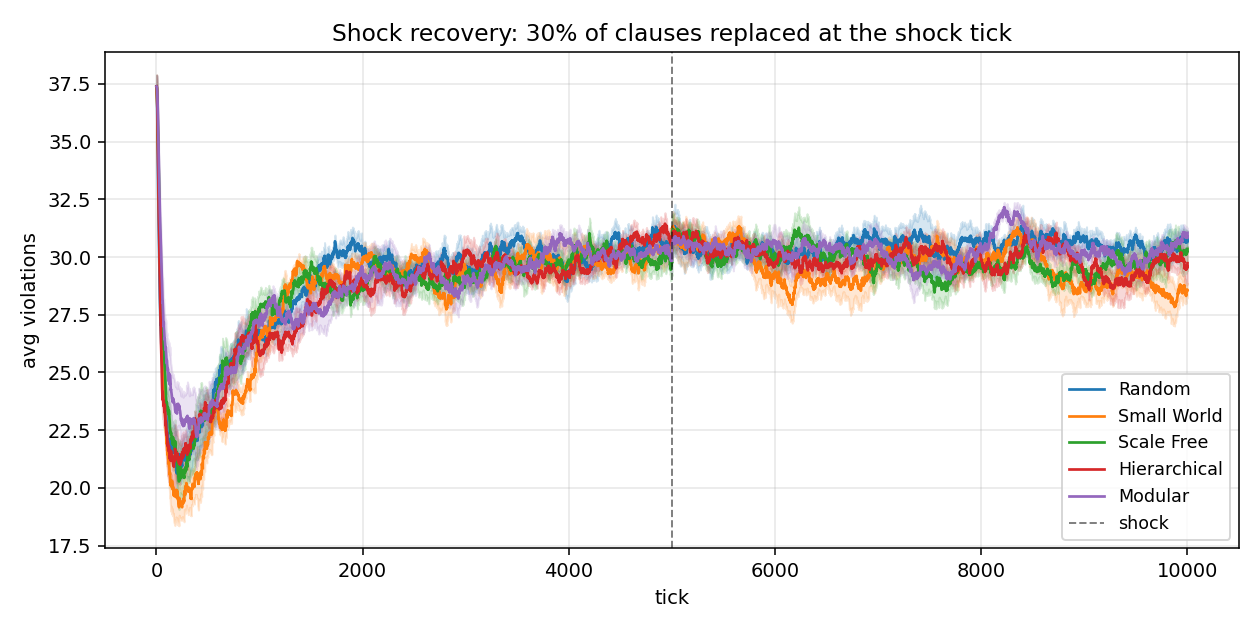
\includegraphics[width=0.85\linewidth]{output/figures/shock_recovery.png}
 \caption{Average violations around a clause-set perturbation at $t=5000$ (vertical dashed line). $30\%$ of the universal clause set is replaced at once. The five topologies differ noticeably in both their initial response (peak jump) and recovery dynamics.}
   \label{fig:shock}
\end{figure}

The shock results recapitulate the asymmetry observed in the unperturbed transient: hierarchical and small-world networks recover faster (their faster-mixing channels propagate the new constraints quickly), modular networks recover most slowly, and the random and scale-free networks lie between the two. Notably, the rank-ordering of topologies under shock recovery is essentially the same as the rank-ordering under initial convergence --- suggesting that ``recoverability'' and ``trainability'' are governed by the same structural features of the network, principally its diameter and the presence of fast cross-cluster paths.

\subsection{Why steady-state equivalence does not contradict structural differentiation}

The combined picture --- topology-insensitive long-run means but topology-sensitive transient behaviour --- is intuitive once stated. Our communication-rate normalisation removes the dominant ``raw bandwidth'' channel by which networks could differentiate themselves, leaving structural advantages and disadvantages that act primarily on \emph{when} information arrives at each agent and not on \emph{how much} arrives in aggregate.

In the long run, each agent's knowledge base converges toward a sample of the global clause distribution, regardless of which neighbours supplied which clauses; this convergence is a consequence of the network's connectivity (every agent eventually inherits content from every other via a chain of communications) and of the additional independent freshness pump provided by the private observation channel. As a result, the long-run distribution of agent states is largely topology-invariant.

In the transient, however, this asymptotic convergence has not yet completed, and the rate at which it does depends on how quickly information can propagate. Hierarchical structures with strong intra-layer mixing and short cross-layer paths reach a nearly-uniform content distribution faster than modular structures whose between-community paths are sparse, even when both are normalised to the same average communication rate.

\subsection{Robustness}

We confirm that the qualitative pattern is preserved under variation of the model parameters. Section~A of the supplementary material reports sweeps of the clause-density parameter $\alpha$, the observation probability $p_{\text{obs}}$, and the clause-replacement interval $\tau$. Across these ranges, the steady-state ordering of topologies on $\bar V^{\text{true}}$ is essentially preserved (modular consistently worse, others within noise of each other), and the transient ordering on $t_{\text{conv}}$ is also preserved (hierarchical fastest, modular slowest).


\section{Discussion and Conclusions}\label{sec:conclusion}

We have shown that under a communication-rate normalisation that controls for raw bandwidth, the long-run aggregate performance of canonical network topologies is remarkably similar; meaningful differences emerge in the transient regime, where the rate of information propagation determines convergence speed, peak descent rate, and recovery from environmental shocks. Two implications are worth drawing out.

\paragraph{Reframing the network--performance question.} A long-standing claim in organisational theory --- that hierarchical structures are uniquely efficient for problem-solving \parencite{simon1962architecture, bolton1994firm} --- often rests on aggregate performance comparisons that conflate communication volume with communication structure. Once volume is held fixed, the apparent superiority of hierarchies in steady state vanishes. What survives is the speed advantage in the transient, which our results connect explicitly to the network's mixing time. Hierarchical organisations are not better at solving a problem; they are faster at adapting to it.

\paragraph{Volatility determines what architecture matters for.} If the constraint environment is stable enough that the system spends most of its time in equilibrium, the choice of architecture is largely a choice over the distribution of work across agents and the homogeneity of solutions, not over aggregate performance. If the environment is volatile --- frequent shocks, rapid drift --- the system spends much of its time in the transient phase, and the architectural differences in convergence speed and recovery time become operationally decisive. Our shock-perturbation results are intended to make this point concrete: under disruption, hierarchical and small-world topologies recover most quickly, while modular ones absorb the perturbation but resolve it slowly.

\paragraph{Trade-offs by topology.} Across our metrics, three loose archetypes emerge:
\begin{itemize}
    \item \textbf{Speed-favouring architectures} (hierarchical, small-world): fast initial convergence, fast recovery from shocks, but no advantage in steady state and limited resilience to losing a key structural feature.
    \item \textbf{Stability-favouring architectures} (modular): slow convergence, slow recovery, but steady-state stability and clear inter-group autonomy.
    \item \textbf{Balanced architectures} (random, scale-free): no extremes, no clear advantage on any single metric, but no clear disadvantage either.
\end{itemize}

\paragraph{Limitations and future work.} Three caveats are worth noting. First, our model deliberately holds individual cognitive abilities homogeneous across agents to isolate the topological contribution; introducing heterogeneous agents (different memory sizes, different greedy intensities, different observation rates) would interact with topology in ways our model cannot predict. Second, our communication-rate normalisation assumes that communication bandwidth is a centrally manageable resource that an organisation chooses to allocate equally across agents; in many real settings, bandwidth is endogenous and concentrates on the agents who provide most value, generating self-reinforcing inequalities that our control rules out. Third, the ``shock'' we model is a homogeneous perturbation of the universal constraint set; in practice, shocks are often localised, and the interaction between localised shocks and modular network structure --- where the shock might affect only some communities directly --- is left for future work.

We expect that the framework developed here can be applied to other domains where interaction networks and node-level role labels are jointly available --- corporate hierarchies, ant-colony task allocation, scientific collaboration networks --- to build a comparative picture of how architecture and dynamics interact across systems where the distinction between ``volume'' and ``structure'' of communication is meaningful.


\section{Acknowledgments}

The authors would like to thank the faculty at Complexity Global School 2025 held at Bogot\'a, Colombia, organised by the Santa Fe Institute and Universidad de Los Andes. We are particularly grateful to Juan Restrepo for methodological guidance, to Emma Zajdela for advice on conference data, and to Joan Kim at the Santa Fe Institute for assistance with the ARCH dataset. Brainstorming with Daniel Torres shaped the project in its early stage, and conversations with Joseph Bak-Coleman in Bogot\'a significantly informed our literature survey.


\printbibliography

\appendix

\section{Implementation details}

The agent-based model is implemented in Python (NumPy, NetworkX, Mesa~3.x). The full source code, including the analysis script that produced all figures and tables in this paper, is provided in the supplementary material.

The communication-scale normalisation is computed once at network construction:
$$
s = 1\,/\,\langle k_{\text{in}}\rangle,
$$
where $\langle k_{\text{in}}\rangle$ is the average in-strength across all $N$ agents. Because all edges carry weight 1, in-strength reduces to in-degree. The per-tick per-edge firing probability is then $\min(1, s \cdot w_{ji})$, which simplifies to $\min(1, 1/\langle k_{\text{in}}\rangle)$ for our uniform-weight networks --- a constant probability across all edges of a given network.

\section{Sensitivity analyses}

Repeats of the main analysis at $\alpha\in\{1,2,4\}$, $p_{\text{obs}}\in\{0.001,0.01,0.05\}$, $\tau\in\{1,10,50\}$ are documented in the supplementary spreadsheet. The qualitative patterns (steady-state convergence across topologies; transient asymmetry favouring hierarchical) are preserved across all explored regimes.


\end{document}
